\chapter{Diseño del proyecto}\label{cap3}
Conforme a lo visto en el capítulo anterior, el proyecto requiere ser ejecutado de dos formas distintas (ejecución de automatizaciones y portal de usuario), además necesita de una base de datos para mantener persistentes los datos de las órdenes de reposición atendidas, catálogos y datos de usuario, también es necesario acceso al sistema de archivo para guardar las capturas de pantalla de las órdenes de reposición enviadas. Por lo que es necesario dos ambientes de ejecución, la automatización que será ejecutada exclusivamente en el sistema operativo y la del web, que si bien también estará contenida en el sistema operativo es necesario que se ejecute parte del sistema en el explorador del usuario.


%===============================================================================
%===============================================================================


\section{Diseño de la arquitectura}
Bourque define la arquitectura de software como:\footnote{\textcolor{red}{Karla, como es cita textual (según mi propia traducción :P ) prefiero dejarla en un párrafo por separado mientras que lo que sea paráfrasis dejarlo en texto seguido ¿cómo ves?}}
\begin{quote}
	El conjunto de estructuras necesarias para la comprensión de un sistema en el cual se comprometen elementos de software, relaciones entre ellos y sus propiedades\cite{SWEBOOK}.
\end{quote}
En las últimas décadas la arquitectura de software ha profundizado en el estudio genérico de las estructuras del software, dando lugar a técnicas como los Patrones de Diseño (ver Apéndice \ref{sec-patrones}) \cite{SWEBOOK, SoftwareArchitectureInAction}.

\textcolor{red}{Karla, Quité las secciones de patrones de diseño, arquitectura 4+1, arquitectura orientada a servicios.}\footnote{\textcolor{red}{Karla, no sentí que los conceptos de patrones de diseño y arquitecturas encajara aquí, así que los mandé al apéndice de patrones de diseño y si los necesito durante este capítulo o el siguiente (implementación) nada más haré referencia ¿Qué opinas?}}

Siguiendo el concepto de arquitectura, dado anteriormente, a continuación se muestran los componentes del sistema y como dan solución a los casos de uso del Capítulo \ref{sec:casos-uso}.

\subsection{Componentes del sistema AutoSA}
El diagrama de componentes sirve para visualizar los componentes en los que se divide el sistema y las interfaces por las cuales se comunican tales componentes, el la Figura \ref{fig:dia-components} se muestra el diagrama de componentes para el sistema AutoSA. En las secciones consecuentes se describe cada componente y las interfaces que ofrece\footnote{Únicamente se mostrarán los diagramas de secuencia más completos que reflejan un comportamiento no trivial.}.
\begin{figure}[h]
\centering
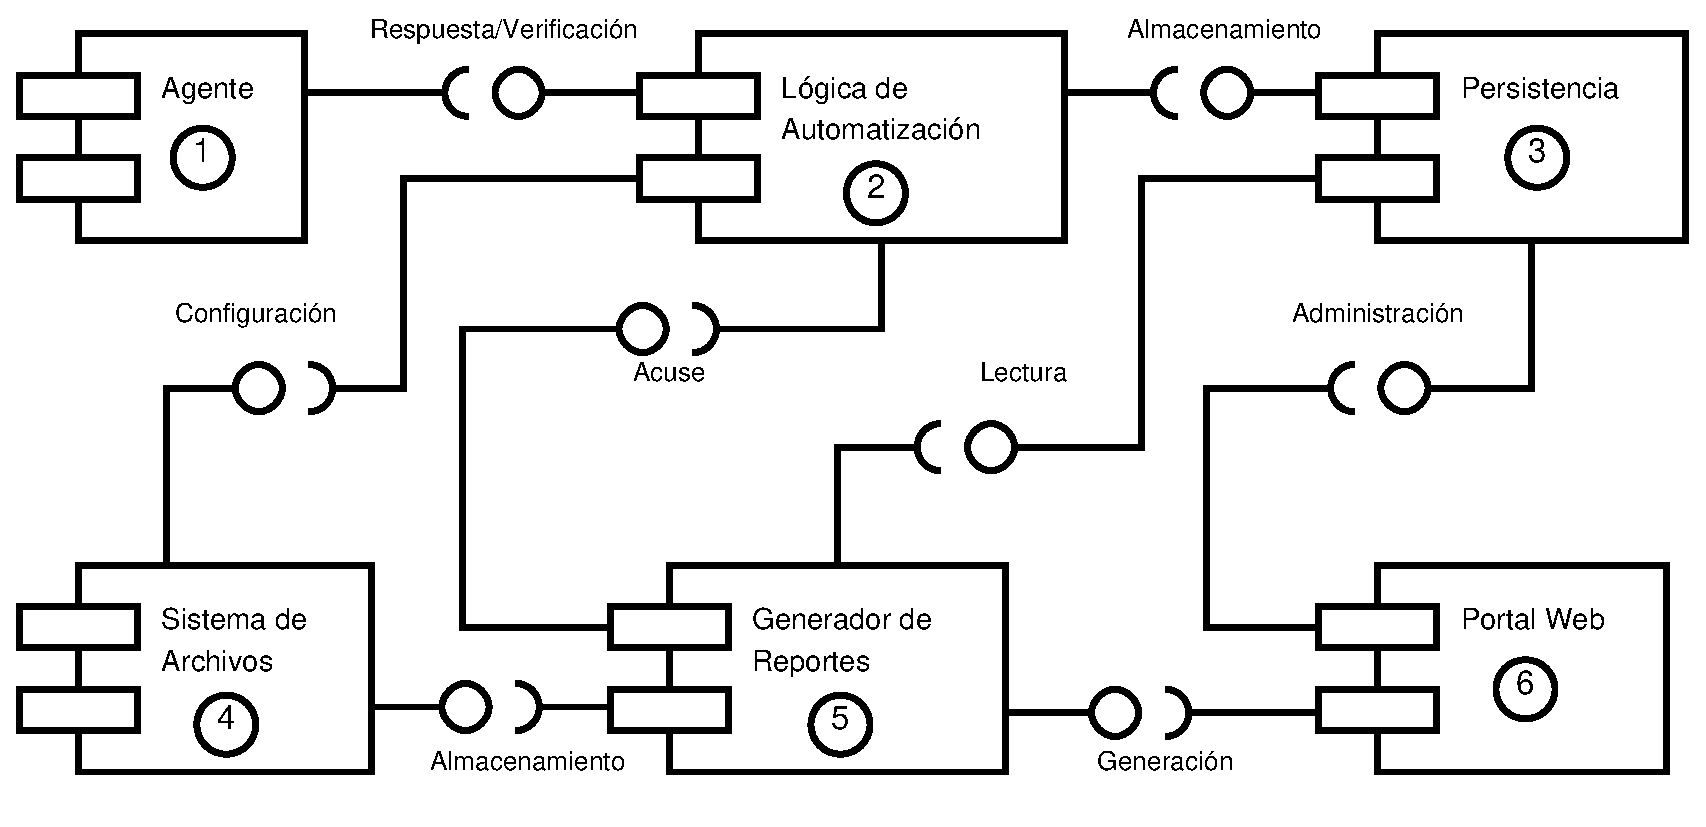
\includegraphics[width=\textwidth]{dia-components}
\caption{Diagrama de componentes.}
\label{fig:dia-components}
\end{figure}

\subsubsection{Agente}
El componente que contiene y ejecuta las rutinas de automatización, esto es mediante una interfaz con el usuario en la cual puede seleccionar el proceso a ser ejecutado. No ofrece interfaces a los demás componentes, consume exclusivamente el componente de Lógica de Automatización.

\subsubsection{Lógica de Automatización}
La función de este componente es de ejecutar las reglas de negocio necesarias para en los flujos de los procesos de automatización.  
\paragraph{Respuesta\\}
Provee el acceso a las reglas de negocio del proceso de respuesta de órdenes de reposición (ver caso de uso \ref{cu-contestar}).\\
\noindent
	\begin{tabular}{|p{\dimexpr.2\textwidth}|p{\dimexpr.8\textwidth-4\tabcolsep}|}
		\hline
		\textbf{Identificador}	& \textbf{guardar-orden-nueva}\\
		\hline
		\hline
		\textbf{Descripción}	& Guarda un listado de nuevas órdenes de reposición.\\
		\hline
		\textbf{Parámetros}		& \textbullet\, Listado de mapas, cada mapa contiene los datos de una orden de reposición.\\
		\hline
		\textbf{Resultado}		& No ofrece resultado.\\
		\hline
	\end{tabular}
	\vspace{3mm}\\
	\begin{tabular}{|p{\dimexpr.2\textwidth}|p{\dimexpr.8\textwidth-4\tabcolsep}|}
		\hline
		\textbf{Identificador}	& \textbf{obtener-orden-contestar}\\
		\hline
		\hline
		\textbf{Descripción}	& Da la siguiente orden de reposición para contestar.\\
		\hline
		\textbf{Parámetros}		& \textbullet\, No recibe parámetros.\\
		\hline
		\textbf{Resultado}		& Mapa con la información de la orden de reposición.\\
		\hline
	\end{tabular}
	\begin{longtable}{|p{\dimexpr.2\textwidth}|p{\dimexpr.8\textwidth-4\tabcolsep}|}
		\hline
		\textbf{Identificador}	& \textbf{obtener-datos-respuesta}\\
		\hline
		\hline
		\textbf{Descripción}	& Da los datos necesarios para llenar los formularios para contestar una orden de reposición en el Sistema de Abastecimiento.\\
		\hline
		\textbf{Parámetros}		& \textbullet\, Mapa con los datos de la orden para contestar.\\
		\hline
		\textbf{Resultado}		& Mapa con la información para llenar los formularios para contestar la orden de reposición.\\
		\hline
	\end{longtable}
	\begin{longtable}{|p{\dimexpr.2\textwidth}|p{\dimexpr.8\textwidth-4\tabcolsep}|}
		\hline
		\textbf{Identificador}	& \textbf{actualizar-orden-contestada}\\
		\hline
		\hline
		\textbf{Descripción}	& Actualiza los datos guardados de la orden de reposición con los datos de la respuesta en el  Sistema de Abastecimiento. Utiliza el componente de persistencia para actualizar los datos.\\
		\hline
		\multirow{2}{*}{\textbf{Parámetros}}	& \textbullet\, Número de orden.\\
												& \textbullet\, Mapa con los datos para guardar.\\
		\hline
		\textbf{Resultado}		& No ofrece resultado.\\
		\hline
	\end{longtable}
	\begin{longtable}{|p{\dimexpr.2\textwidth}|p{\dimexpr.8\textwidth-4\tabcolsep}|}
		\hline
		\textbf{Identificador}	& \textbf{obtener-orden-enviar}\\
		\hline
		\hline
		\textbf{Descripción}	& Da la siguiente orden de reposición para enviar.\\
		\hline
		\textbf{Parámetros}		& \textbullet\, No recibe parámetros.\\
		\hline
		\textbf{Resultado}		& Mapa con la información de la orden de reposición.\\
		\hline
	\end{longtable}
	\begin{longtable}{|p{\dimexpr.2\textwidth}|p{\dimexpr.8\textwidth-4\tabcolsep}|}
		\hline
		\textbf{Identificador}	& \textbf{guardar-orden-enviada}\\
		\hline
		\hline
		\textbf{Descripción}	& Actualiza los datos guardados de la orden de reposición con los datos de la pantalla de envío del Sistema de Abastecimiento. Utiliza el componente de persistencia para actualizar los datos.\\
		\hline
		\multirow{2}{*}{\textbf{Parámetros}}	& \textbullet\, Número de orden.\\
												& \textbullet\, Mapa con los datos para guardar.\\
		\hline
		\textbf{Resultado}		& No ofrece resultado.\\
		\hline
	\end{longtable}
	\begin{longtable}{|p{\dimexpr.2\textwidth}|p{\dimexpr.8\textwidth-4\tabcolsep}|}
		\hline
		\textbf{Identificador}	& \textbf{obtener-acuse-envio}\\
		\hline
		\hline
		\textbf{Descripción}	& Solicita la generación de el acuse de envío al componente de reportes y almacena el documento el componente de Sistema de Archivos.\\
		\hline
		\textbf{Parámetros}		& \textbullet\, Número de orden.\\
		\hline
		\textbf{Resultado}		& No ofrece resultado.\\
		\hline
	\end{longtable}
	\vspace{5mm}
\paragraph{Verificación\\}
Provee el acceso a las reglas de negocio del proceso de verificación de órdenes de reposición canceladas.

	\begin{longtable}{|p{\dimexpr.2\textwidth}|p{\dimexpr.8\textwidth-4\tabcolsep}|}
		\hline
		\textbf{Identificador}	& \textbf{obtener-rango-verificar}\\
		\hline
		\hline
		\textbf{Descripción}	& Obtiene el rango de fechas para ingresar en el formulario de búsqueda del Sistema de Abastecimiento. El número de días que comprende el rango se obtiene utilizando el componente de Sistema de archivos.\\
		\hline
		\textbf{Parámetros}		& \textbullet\, No tiene parámetros.\\
		\hline
		\textbf{Resultado}		& El número de días para el rango de búsqueda.\\
		\hline
	\end{longtable}

	\begin{longtable}{|p{\dimexpr.2\textwidth}|p{\dimexpr.8\textwidth-4\tabcolsep}|}
		\hline
		\textbf{Identificador}	& \textbf{actualizar-estado-sa}\\
		\hline
		\hline
		\textbf{Descripción}	& Actualiza el EstadoSA de las órdenes de reposición recibidas a \textbf{Cancelada}. Utiliza el componente de persistencia para la actualización de datos.\\
		\hline
		\textbf{Parámetros}		& \textbullet\, Listado con los números de las órdenes de reposición canceladas.\\
		\hline
		\textbf{Resultado}		& El número de órdenes de reposición actualizadas.\\
		\hline
	\end{longtable}

\subsubsection{Persistencia}
El componente de persistencia está basado en el patrón de diseño \textit{DAO}(ver apéndice \ref{sec-dao}) para controlar el acceso a la base de datos\footnote{En adelante se utilizará \textbf{DAO} para hacer referencia al patrón y la instancia (objeto) del patrón.}.\\
El componente de persistencia de el proyecto AutoSA presenta las siguientes interfaces de búsqueda y almacenamiento:
\paragraph{Almacenamiento\\}
Conjunto de operaciones diseñadas para responder a las necesidades de almacenamiento en los flujos para responder y verificar órdenes de reposición\footnote{Ver casos de uso \ref{cu-contestar}, \ref{cu-guardar-nueva}, \ref{cu-responder-orden}, \ref{cu-enviar-orden} y \ref{cu-actualizar-estatus-sa}.}:

	\begin{longtable}{|p{\dimexpr.2\textwidth}|p{\dimexpr.8\textwidth-4\tabcolsep}|}
		\hline
		\textbf{Identificador}	& \textbf{guardar-nueva} \\
		\hline
		\hline
		\textbf{Descripción}	& Inserta una nueva orden de reposición en la base de datos.\\
		\hline
		\textbf{Parámetros} 	& \textbullet\, Mapa con los datos de la orden de reposición.\\
		\hline
		\textbf{Resultado}		& No ofrece resultado.\\
		\hline
	\end{longtable}

	\begin{longtable}{|p{\dimexpr.2\textwidth}|p{\dimexpr.8\textwidth-4\tabcolsep}|}
		\hline
		\textbf{Identificador}	& \textbf{cambiar-estado} \\
		\hline
		\hline
		\textbf{Descripción}	& Cambia el estado de atención de una orden de reposición. \\
		\hline
		\multirow{2}{*}{\textbf{Parámetros}}	& \textbullet\, Número de orden de reposición.\\
												& \textbullet\, Estado.\\
		\hline
		\textbf{Resultado}		& No ofrece resultado.\\
		\hline
	\end{longtable}

	\begin{longtable}{|p{\dimexpr.2\textwidth}|p{\dimexpr.8\textwidth-4\tabcolsep}|}
		\hline
		\textbf{Identificador}	& \textbf{guardar-respuesta}\\
		\hline
		\hline
		\textbf{Descripción}	& Guarda los datos de los formularios de la pantalla de respuesta de las órdenes de reposición.\\
		\hline
		\multirow{2}{*}{\textbf{Parámetros}}	& \textbullet\, Número de orden de reposición.\\
												& \textbullet\, Mapa con los datos de los formularios.\\
		\hline
		\textbf{Resultado}		& No ofrece resultado.\\
		\hline
	\end{longtable}

	\begin{longtable}{|p{\dimexpr.2\textwidth}|p{\dimexpr.8\textwidth-4\tabcolsep}|}
		\hline
		\textbf{Identificador}	& \textbf{guardar-folio-acuse}\\
		\hline
		\hline
		\textbf{Descripción}	& Guarda el folio de acuse de envío de la orden de reposición.\\
		\hline
		\multirow{2}{*}{\textbf{Parámetros}} 	& \textbullet\, Número de orden de reposición.\\
												& \textbullet\, Folio de acuse de envío.\\
		\hline
		\textbf{Resultado}		& No ofrece resultado.\\
		\hline
	\end{longtable}

	\begin{longtable}{|p{\dimexpr.2\textwidth}|p{\dimexpr.8\textwidth-4\tabcolsep}|}
		\hline
		\textbf{Identificador}	& \textbf{actualizar-estado-sa}\\
		\hline
		\hline
		\textbf{Descripción}	& Actualiza el estado de atención en el Sistema de Abastecimiento a \textbf{cancelada} de las órdenes de reposición recibidas.\\
		\hline
		\textbf{Parámetros} 	& \textbullet\, Lista con los números de las órdenes de reposición.\\
		\hline
		\textbf{Resultado}		& El número de órdenes de reposición actualizadas.\\
		\hline
	\end{longtable}

	\begin{longtable}{|p{\dimexpr.2\textwidth}|p{\dimexpr.8\textwidth-4\tabcolsep}|}
		\hline
		\textbf{Identificador}	& \textbf{registrar-evento}\\
		\hline
		\hline
		\textbf{Descripción}	& Registra en la base de datos un evento que ocurre durante los procesos automatizados, el evento puede ser de carácter informativo o de error.\\
		\hline
		\multirow{2}{*}{\textbf{Parámetros}}	& \textbullet\, Tipo de evento.\\
												& \textbullet\, Mapa con la descripción del evento.\\
		\hline
		\textbf{Resultado}		& No ofrece resultado.\\
		\hline
	\end{longtable}

\paragraph{Lectura\\}
Conjunto de operaciones diseñadas para las necesidades de lectura de órdenes de reposición en los flujos para responder y verificar órdenes de reposición\footnote{Ver casos de uso \ref{cu-contestar}, \ref{cu-enviar-orden} y \ref{cu-generar-acuse}.}:

	\begin{longtable}{|p{\dimexpr.2\textwidth}|p{\dimexpr.8\textwidth-4\tabcolsep}|}
		\hline
		\textbf{Identificador}	& \textbf{siguiente-orden-contestar}\\
		\hline
		\hline
		\textbf{Descripción}	& Entrega un mapa con los datos de la primera orden de reposición encontrada con estado \textbf{Nueva}.\\
		\hline
		\textbf{Parámetros} 	& \textbullet\, No tiene parámetros.\\
		\hline
		\textbf{Resultado}		& Un mapa con los datos de la primera orden de reposición encontrada con estado \textbf{Nueva}. En caso de no existir tal orden regresa un mapa vacío.\\
		\hline
	\end{longtable}

	\begin{longtable}{|p{\dimexpr.2\textwidth}|p{\dimexpr.8\textwidth-4\tabcolsep}|}
		\hline
		\textbf{Identificador}	& \textbf{siguiente-orden-enviar}\\
		\hline
		\hline
		\textbf{Descripción}	& Entrega un mapa con los datos de la primera orden de reposición encontrada con estado \textbf{Contestada}.\\
		\hline
		\textbf{Parámetros} 	& \textbullet\, No tiene parámetros.\\
		\hline
		\textbf{Resultado}		& Un mapa con los datos de la primera orden de reposición encontrada con estado \textbf{Contestada}. En caso de no existir tal orden regresa un mapa vacío.\\
		\hline
	\end{longtable}

	\begin{longtable}{|p{\dimexpr.2\textwidth}|p{\dimexpr.8\textwidth-4\tabcolsep}|}
		\hline
		\textbf{Identificador}	& \textbf{obtener-datos-acuse}\\
		\hline
		\hline
		\textbf{Descripción}	& Obtiene los datos de una orden de reposición necesarios para generar el documento de acuse de envío.\\
		\hline
		\textbf{Parámetros}		& \textbullet\, Número de orden de reposición.\\
		\hline
		\textbf{Resultado}		& Un mapa con los datos de la orden de reposición. En caso de no existir tal orden regresa un mapa vacío.\\
		\hline
	\end{longtable}

\paragraph{Administración\\}
Son las operaciones que permiten modificar datos específicos de las órdenes de reposición contenidas en la base de datos, también ofrece la actualización masiva de catálogos\footnote{Ver casos de uso \ref{cu-entrar-web}, \ref{cu-generar-reporte}, \ref{cu-actualizar-catalogo}, \ref{cu-buscar}, \ref{cu-visualizar} y \ref{cu-editar}.}).

	\begin{longtable}{|p{\dimexpr.2\textwidth}|p{\dimexpr.8\textwidth-4\tabcolsep}|}
		\hline
		\textbf{Identificador}	& \textbf{buscar-credenciales}\\
		\hline
		\hline
		\textbf{Descripción}	& Busca las credenciales del usuario.\\
		\hline
		\textbf{Parámetros}		& \textbullet\, Identificador de usuario.\\
		\hline
		\textbf{Resultado}		& Un mapa con las credenciales del usuario.\\
		\hline
	\end{longtable}

	\begin{longtable}{|p{\dimexpr.2\textwidth}|p{\dimexpr.8\textwidth-4\tabcolsep}|}
		\hline
		\textbf{Identificador}	& \textbf{extraer-reporte}\\
		\hline
		\hline
		\textbf{Descripción}	& Ejecuta la búsqueda necesaria para extraer los datos del reporte indicado.\\
		\hline
		\multirow{2}{*}{\textbf{Parámetros}}	& \textbullet\, Tipo de reporte.\\
												& \textbullet\, Mapa con los parámetros del filtro de búsqueda.\\
		\hline
		\textbf{Resultado}		& Un listado con los datos del reporte.\\
		\hline
	\end{longtable}

	\begin{longtable}{|p{\dimexpr.2\textwidth}|p{\dimexpr.8\textwidth-4\tabcolsep}|}
		\hline
		\textbf{Identificador}	& \textbf{actualizar-catalogo}\\
		\hline
		\hline
		\textbf{Descripción}	& Actualiza la información del catálogo indicado.\\
		\hline
		\multirow{2}{*}{\textbf{Parámetros}}	& \textbullet\, Identificador del catálogo.\\
												& \textbullet\, Listado con los datos del catálogo.\\
		\hline
		\textbf{Resultado}		& El número de los registros insertados en el catálogo.\\
		\hline
	\end{longtable}

	\begin{longtable}{|p{\dimexpr.2\textwidth}|p{\dimexpr.8\textwidth-4\tabcolsep}|}
		\hline
		\textbf{Identificador}	& \textbf{buscar-ordenes}\\
		\hline
		\hline
		\textbf{Descripción}	& Busca órdenes de reposición que cumplan con el filtro de búsqueda indicado.\\
		\hline
		\textbf{Parámetros}		& \textbullet\, Mapa con el filtro de búsqueda.\\
		\hline
		\textbf{Resultado}		& Un listado con las órdenes de reposición encontradas.\\
		\hline
	\end{longtable}

	\begin{longtable}{|p{\dimexpr.2\textwidth}|p{\dimexpr.8\textwidth-4\tabcolsep}|}
		\hline
		\textbf{Identificador}	& \textbf{buscar-orden}\\
		\hline
		\hline
		\textbf{Descripción}	& Busca una orden de reposición por el número de orden.\\
		\hline
		\textbf{Parámetros}		& \textbullet\, Número de orden de reposición.\\
		\hline
		\textbf{Resultado}		& La orden de reposición encontrada. En caso de no encontrar la orden se regresa un identificador vacío.\\
		\hline
	\end{longtable}

	\begin{longtable}{|p{\dimexpr.2\textwidth}|p{\dimexpr.8\textwidth-4\tabcolsep}|}
		\hline
		\textbf{Identificador}	& \textbf{actualizar-orden}\\
		\hline
		\hline
		\textbf{Descripción}	& Actualiza los datos de orden de reposición.\\
		\hline
		\multirow{2}{*}{\textbf{Parámetros}}	& \textbullet\, Número de orden.\\
												& \textbullet\, Mapa con los datos actualizados.\\
		\hline
		\textbf{Excepciones}	& Error si la orden de reposición no se encuentra registrada en la base de datos.\\
		\hline
	\end{longtable}

\subsubsection{Sistema de Archivos}
El componente Sistema de Archivos es el único que se comunica con el sistema de archivos del sistema operativo\footnote{En este documento se utilizará de forma indistinta el término Sistema de archivos para referirse tanto al componente del sistema AutoSA como al propio del sistema operativo.}, tiene la función de realizar la lectura de archivos de configuración, el almacenamiento de los acuses de envío  y los reportes de las órdenes de reposición.\\
Este componente también está diseñado siguiendo el patrón DAO\footnote{Ver apéndice \ref{sec-dao}}.
\paragraph{Configuración\\}
Da la configuración contenida en archivos de propiedades contenidas en el mismo sistema de archivos.

	\begin{longtable}{|p{\dimexpr.2\textwidth}|p{\dimexpr.8\textwidth-4\tabcolsep}|}
		\hline
		\textbf{Identificador}	& \textbf{obtener-propiedad}\\
		\hline
		\hline
		\textbf{Descripción}	& Obtiene una propiedad de los archivos de configuración.\\
		\hline
		\textbf{Parámetros}		& \textbullet\, Identificador de la propiedad.\\
		\hline
		\textbf{Resultado}		& El valor de la propiedad. Si no existe la propiedad regresa la cadena vacía.\\
		\hline
	\end{longtable}

\paragraph{Almacenamiento\\}
Almacena archivos (reportes y acuses de envío) en el sistema de archivos.

	\begin{longtable}{|p{\dimexpr.2\textwidth}|p{\dimexpr.8\textwidth-4\tabcolsep}|}
		\hline
		\textbf{Identificador}	& \textbf{guardar-archivo}\\
		\hline
		\hline
		\textbf{Descripción}	& Guarda un archivo en el sistema de archivos.\\
		\hline
		\multirow{2}{*}{\textbf{Parámetros}}	& \textbullet\, Archivo.\\
												& \textbullet\, Ruta del archivo.\\
		\hline
		\textbf{Resultado}		& No ofrece resultado.\\
		\hline
	\end{longtable}

\subsubsection{Generador de Reportes}
El Generador de Reportes, como su nombre lo indica, tiene la función de generar documentos y reportes con los datos de las órdenes de reposición almacenados en la base de datos. 
\paragraph{Acuse\\} Genera el documento con el acuse de envío.

	\begin{longtable}{|p{\dimexpr.2\textwidth}|p{\dimexpr.8\textwidth-4\tabcolsep}|}
		\hline
		\textbf{Identificador}	& \textbf{generar-acuse-envio}\\
		\hline
		\hline
		\textbf{Descripción}	& Genera el acuse de envío para la orden de reposición especificada. Utiliza el componente de persistencia para obtener los datos de la orden.\\
		\hline
		\textbf{Parámetros}		& \textbullet\, Número de la orden de reposición.\\
		\hline
		\textbf{Resultado}		& La ruta en el sistema de archivos donde ha sido depositado el acuse de envío.\\
		\hline
	\end{longtable}

\paragraph{Generación\\} Genera reportes con los datos de las órdenes de reposición almacenados en la base de datos.

	\begin{longtable}{|p{\dimexpr.2\textwidth}|p{\dimexpr.8\textwidth-4\tabcolsep}|}
		\hline
		\textbf{Identificador}	& \textbf{generar-reporte-ordenes}\\
		\hline
		\hline
		\textbf{Descripción}	& Genera el reporte del tipo indicado, usando el rango de fechas establecido.\\
		\hline
		\multirow{3}{*}{\textbf{Parámetros}}	& \textbullet\, Tipo de reporte.\\
												& \textbullet\, Fecha inicial.\\
												& \textbullet\, Fecha final.\\
		\hline
		\textbf{Resultado}		& La ruta en el sistema de archivos donde ha sido depositado el reporte generado.\\
		\hline
	\end{longtable}

\subsubsection{Portal Web}
Es componente que ofrece al usuario las funcionalidades de una interfaz web, está diseñado siguiendo el patrón MVC\footnote{Ver sección \ref{sec-mvc}}. Utiliza el componente de persistencia como el modelo, mientras que la vista se toma en dos partes: las pantallas que se muestran al usuario y los reportes, para esta última toma las funciones del componente de Generación de Reportes y Sistema de Archivos.\\
No ofrece interfaces a los demás componentes, al igual que el componente Agente.



\subsection{Solución a casos de uso}
A continuación se presentan las soluciones a los casos de uso utilizando los componentes descritos en la sección anterior, para este fin se utilizan diagramas de secuencia UML\footnote{Ver sección \ref{sec-uml-seq}.}

\subsubsection{Contestar órdenes}
El diseño de la solución al caso de uso \textbf{CU-CONTESTAR} (sección \ref{cu-contestar}) se lleva a cabo entre el actor \textbf{Usuario} y los componentes \textbf{Agente} \textbf{Lógica de Automatización}. La solución sigue la siguiente secuencia (ver diagrama\footnote{Por cuestión del tamaño de la figura y conservar el texto dentro de ella de tamaño legible únicamente se mostrarán los mensajes más importantes entre componentes} de la Figura \ref{fig:dia-seq-cu-contestar}):
\begin{enumerate}
	\item \textbf{Usuario}: inicia la ejecución del agente (mensaje 1 del diagrama).
	\item \textbf{Agente}: dirige el explorador de Internet a la página del Sistema de Abastecimiento y pide al usuario la contraseña para ingresar.
	\item \textbf{Usuario}: proporciona la contraseña (mensaje 2 del diagrama).
	\item \textbf{Agente}: realiza el acceso al Sistema de Abastecimiento
	\item \textbf{Agente}: dirige el explorador de Internet al listado de órdenes de reposición.
	\item \textbf{Agente}: para cada orden en el listado, ejecuta el caso de uso \textbf{CU-GUARDAR-NUEVA} con apoyo del componente \textbf{Lógica de Automatización} (mensaje 3 del diagrama).
	\item \textbf{Agente}: para cada orden con estado \textbf{NUEVA} en la base de datos, ejecuta el caso de uso \textbf{CU-RESPONDER-ORDEN} con apoyo del componente \textbf{Lógica de Automatización} (mensaje 4 del diagrama).
	\item \textbf{Agente}: para cada orden con estado \textbf{CONTESTADA} en la base de datos, ejecuta los casos de uso \textbf{CU-ENVIAR-ORDEN} y \textbf{CU-GENERAR-ACUSE} con apoyo del componente \textbf{Lógica de Automatización} (mensaje 5 del diagrama).
\end{enumerate}

\begin{figure}[h]
	\centering
	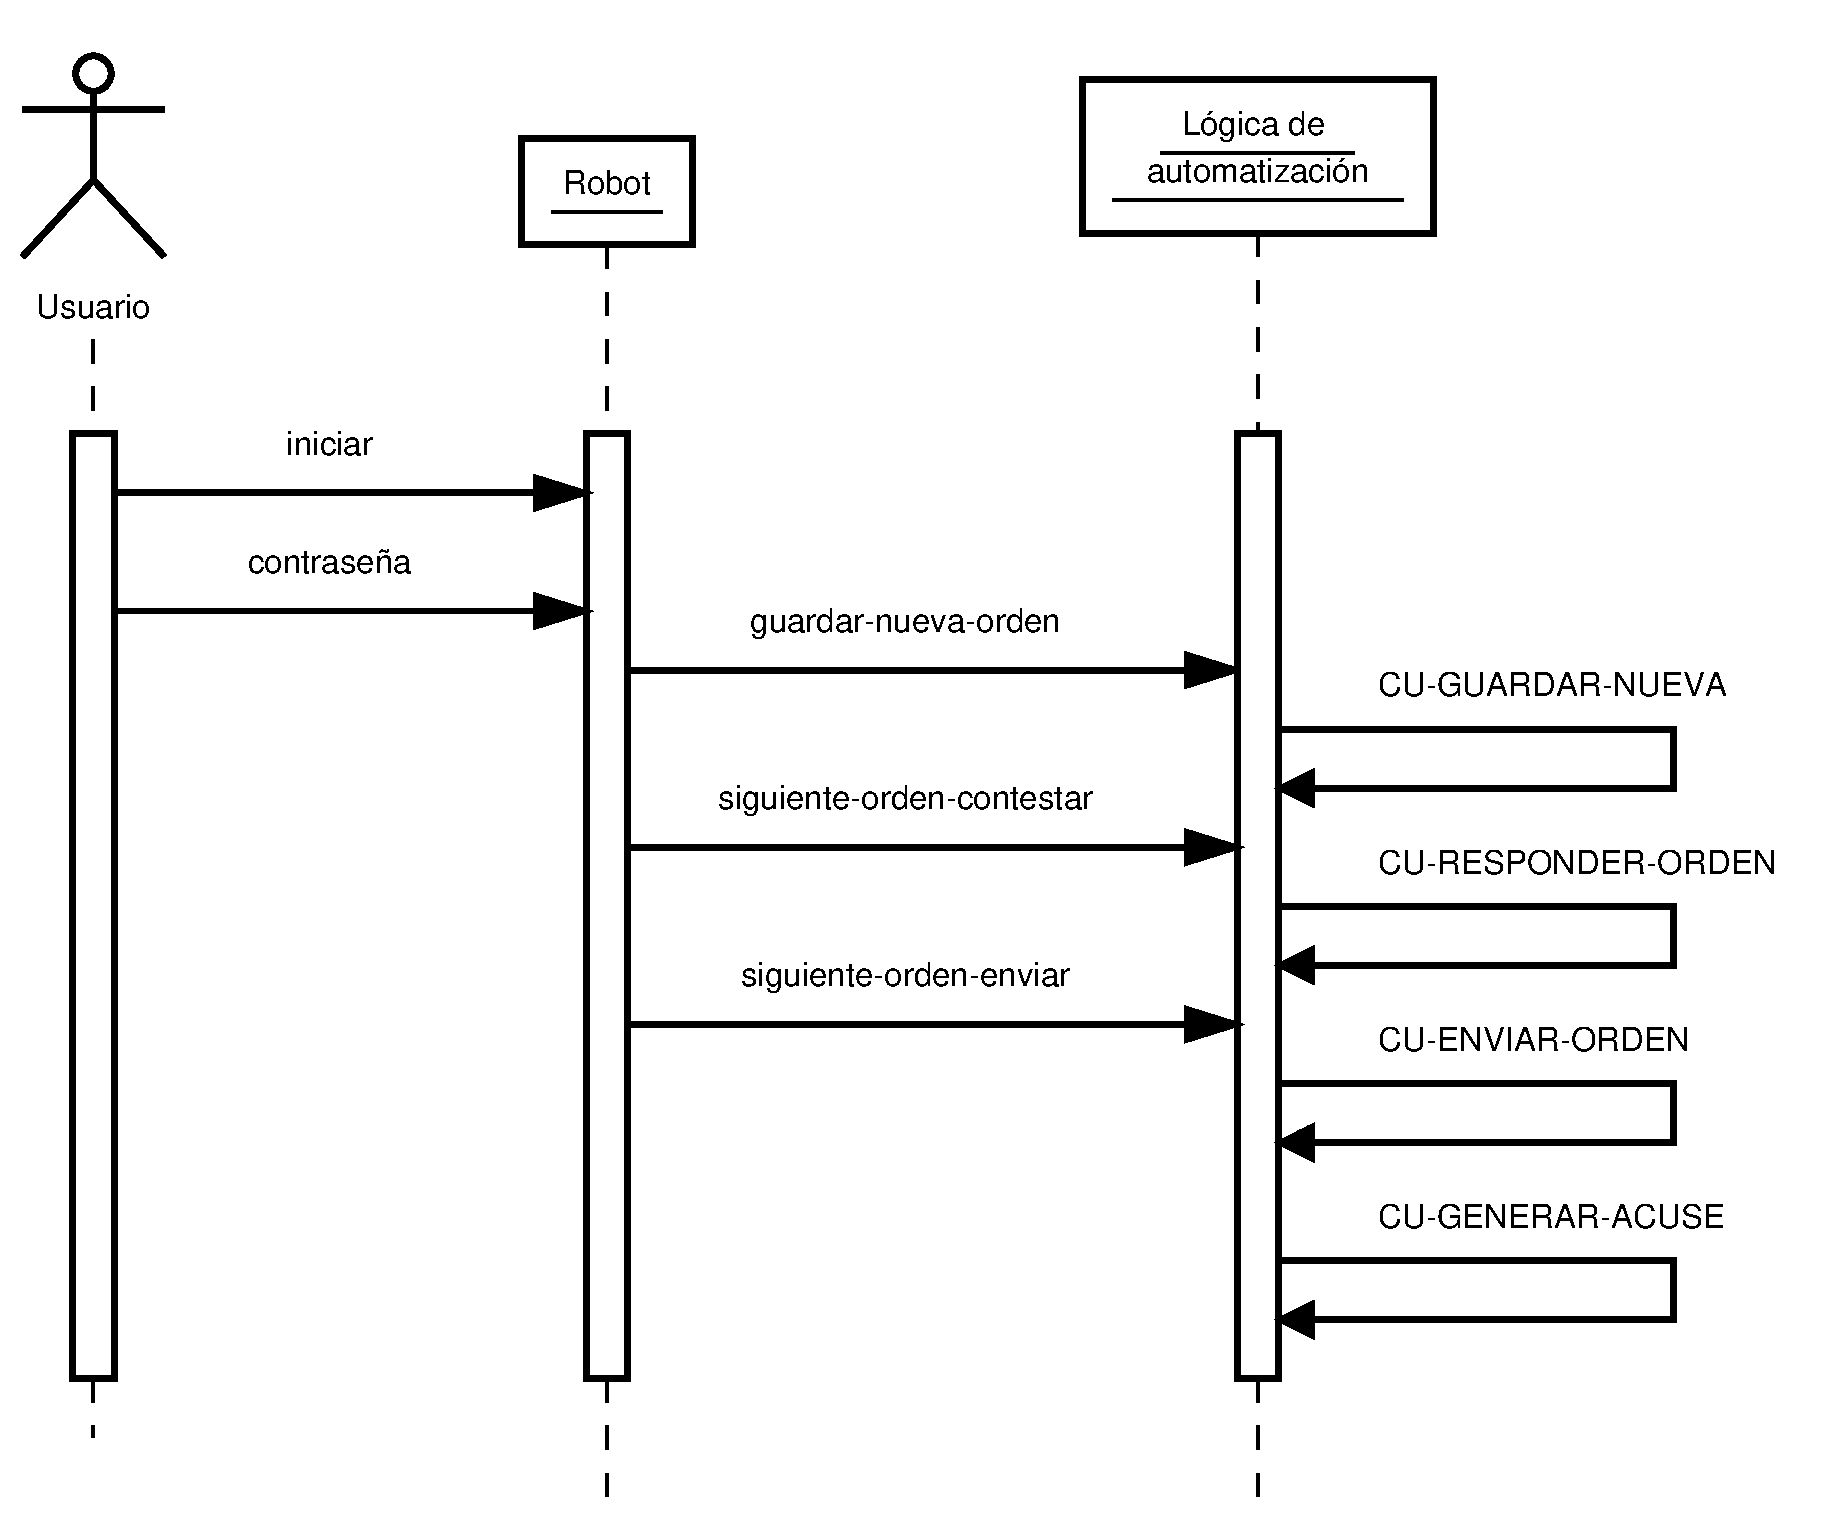
\includegraphics[scale=0.7]{dia-seq-cu-contestar}
	\caption{Diagrama de secuencia del caso de uso CU-CONTESTAR.}
	\label{fig:dia-seq-cu-contestar}
\end{figure}

\subsubsection{Guardar nueva orden}
El diseño para la solución del caso de uso \textbf{CU-GUARDAR-NUEVA} (sección \ref{cu-guardar-nueva}) utiliza los componentes \textbf{Agente}, \textbf{Lógica de Automatización} y \textbf{Persistencia}, tal solución se logra realizando las siguientes llamadas (En el diagrama de la Figura \ref{fig:dia-seq-cu-guardar-nueva} se muestra el diagrama de secuencia.):
\begin{enumerate}
	\item \textbf{Agente}: envía los datos de la nueva orden de reposición (mensaje 1 del diagrama).
	\item \textbf{Lógica de Automatización}: remueve (de encontrarse) los espacios en blanco al principio y al final de cada dato de la orden.
	\item \textbf{Lógica de Automatización}: construye la \textit{URL} de envío de la orden de reposición.
	\item \textbf{Lógica de Automatización}: envía la orden de reposición al componente de persistencia, (mensaje 2 del diagrama).
	\item \textbf{Persistencia}: almacena la orden de reposición en la base de datos.
\end{enumerate}

\begin{figure}[h]
	\centering
	\includegraphics[scale=0.7]{dia-seq-cu-guardar-nueva}
	\caption{Diagrama de secuencia del caso de uso CU-GUARDAR-NUEVA.}
	\label{fig:dia-seq-cu-guardar-nueva}
\end{figure}

\subsubsection{Responder orden}
El diseño para la solución del caso de uso \textbf{CU-RESPONDER-ORDEN} (sección \ref{cu-responder-orden}) utiliza los componentes \textbf{Agente}, \textbf{Lógica de Automatización} y \textbf{Persistencia}, tal solución se logra realizando las siguientes llamadas (En el diagrama de la Figura \ref{fig:dia-seq-cu-responder-orden} se muestra el diagrama de secuencia):
\begin{enumerate}
	\item \textbf{Agente}: pide la siguiente orden de reposición para contestar (mensaje 1 del diagrama).
	\item \textbf{Lógica de Automatización}: consulta el componente \textbf{Persistencia} para obtener la siguiente orden para contestar.
	\item \textbf{Persistencia}: obtiene la primera orden de reposición con estado \textbf{Nueva}.
	\item \textbf{Persistencia}: cambia el estado de la orden a \textbf{Siendo Contestada} (mensaje 3 del diagrama).
	\item \textbf{Agente}: pide los datos para llenar los formularios (mensaje 6 del diagrama).
	\item \textbf{Agente}: pide almacenar los datos de la orden de reposición contestada (mensaje 7 del diagrama).
	\item \textbf{Lógica de Automatización}: envía los datos de la orden contestada al componente \textbf{Persistencia} para que sean almacenados (mensaje 8 del diagrama).
	\item \textbf{Lógica de Automatización}: manda el cambio de estado de la orden a \textbf{Contestada} (mensaje 9 del diagrama).
\end{enumerate}

\begin{figure}[h]
	\centering
	\includegraphics[scale=0.7]{dia-seq-cu-responder-orden}
	\caption{Diagrama de secuencia del caso de uso CU-RESPONDER-ORDEN.}
	\label{fig:dia-seq-cu-responder-orden}
\end{figure}

\subsubsection{Enviar orden}
El diseño para la solución del caso de uso \textbf{CU-ENVIAR-ORDEN} (sección \ref{cu-enviar-orden}) utiliza los componentes \textbf{Agente}, \textbf{Lógica de Automatización} y \textbf{Persistencia}, tal solución se logra realizando las siguientes llamadas (En el diagrama de la Figura \ref{fig:dia-seq-cu-enviar-orden} se muestra el diagrama de secuencia):
\begin{enumerate}
	\item \textbf{Agente}: pide la siguiente orden de reposición para enviar (mensaje 1 del diagrama).
	\item \textbf{Lógica de Automatización}: consulta el componente \textbf{Persistencia} para obtener la siguiente orden para enviar (mensaje 2 del diagrama).
	\item \textbf{Persistencia}: obtiene la primera orden de reposición con estado \textbf{Contestada}.
	\item \textbf{Persistencia}: cambia el estado de la orden a \textbf{Siendo Enviada} (mensaje 3 del diagrama).
	\item \textbf{Agente}: dirige el explorador a la \textit{URL de envío}.
	\item \textbf{Agente}: manda almacenar el folio de envío (mensaje 6 del diagrama).
	\item \textbf{Lógica de Automatización}: utiliza el componente \textbf{Persistencia} para almacenar el folio de envío (mensaje 7 del diagrama).
	\item \textbf{Lógica de Automatización}: actualiza el estado de la orden a \textbf{Enviada} (mensaje 8 del diagrama).
\end{enumerate}

\begin{figure}[h]
	\centering
	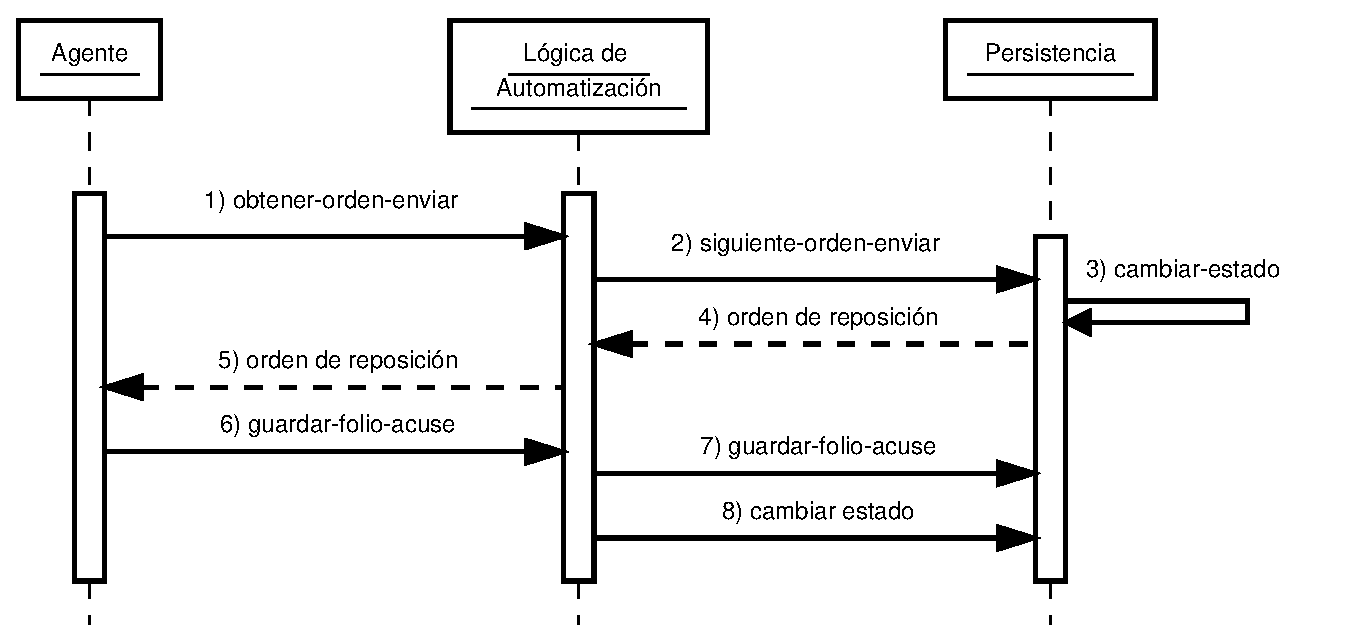
\includegraphics[scale=0.7]{dia-seq-cu-enviar-orden}
	\caption{Diagrama de secuencia del caso de uso CU-ENVIAR-ORDEN.}
	\label{fig:dia-seq-cu-enviar-orden}
\end{figure}

\subsubsection{Generar acuse de envío}
El diseño para la solución del caso de uso \textbf{CU-GENERAR-ACUSE} (sección \ref{cu-generar-acuse}) utiliza los componentes \textbf{Lógica de Automatización}, \textbf{Persistencia}, \textbf{Generador de Reportes} y \textbf{Sistema de Archivos} tal solución se logra realizando las siguientes llamadas (En el diagrama de la Figura \ref{fig:dia-seq-cu-generar-acuse} se muestra el diagrama de secuencia):
\begin{enumerate}
	\item \textbf{Lógica de Automatización}: pide los datos de la orden de reposición al componente \textbf{Persistencia} (mensaje 1 del diagrama).
	\item \textbf{Lógica de Automatización}: pide la generación del acuse de envío al componente \textbf{Generador de Reportes} (mensaje 2 del diagrama).
	\item \textbf{Generador de Reportes}: pide almacenar el acuse de envío al componente \textbf{Sistema de Archivos} (mensaje 3 del diagrama).
\end{enumerate}

\begin{figure}[h]
	\centering
	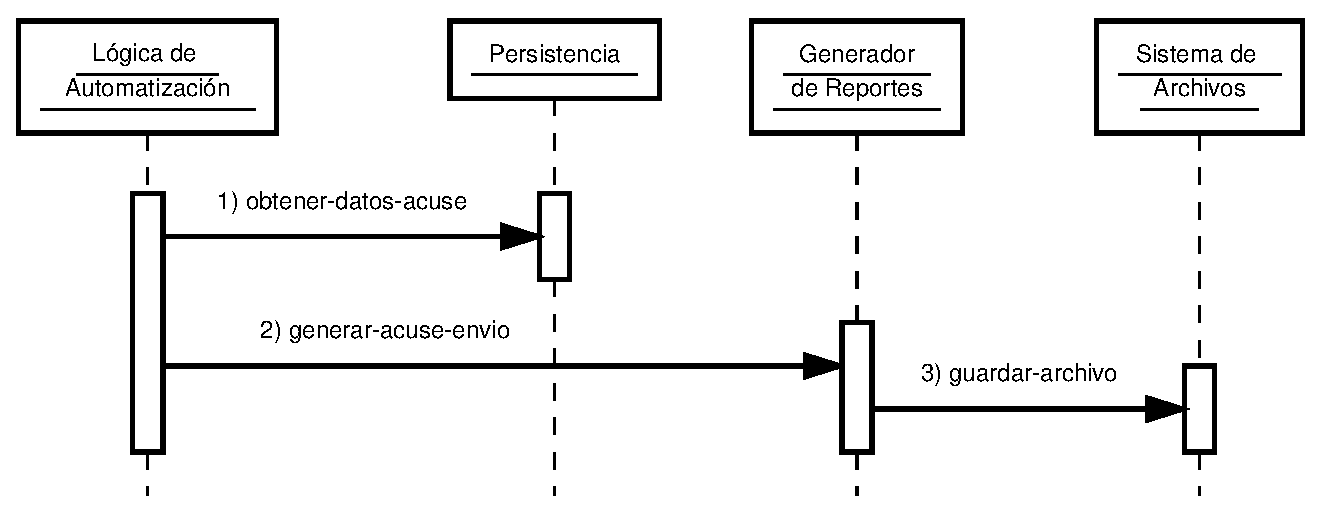
\includegraphics[scale=0.7]{dia-seq-cu-generar-acuse}
	\caption{Diagrama de secuencia del caso de uso CU-GENERAR-ACUSE.}
	\label{fig:dia-seq-cu-generar-acuse}
\end{figure}

\subsubsection{Verificar órdenes}
El diseño de la solución al caso de uso \textbf{CU-VERIFICAR} (sección \ref{cu-verificar}) se lleva a cabo entre el actor \textbf{Usuario} y los componentes \textbf{Agente} \textbf{Lógica de Automatización} tal solución se logra realizando las siguientes llamadas (En el diagrama de la Figura \ref{fig:dia-seq-cu-verificar} se muestra el diagrama de secuencia):
\begin{enumerate}
	\item \textbf{Usuario}: inicia la ejecución del agente (mensaje 1 del diagrama).
	\item \textbf{Agente}: dirige el explorador de Internet a la página del Sistema de Abastecimiento y pide al usuario la contraseña para ingresar.
	\item \textbf{Usuario}: proporciona la contraseña (mensaje 2 del diagrama).
	\item \textbf{Agente}: realiza el acceso al Sistema de Abastecimiento
	\item \textbf{Agente}: dirige el explorador de Internet a la búsqueda de órdenes de reposición.
	\item \textbf{Agente}: pide el rango de fechas al componente \textbf{Lógica de Automatización} (mensaje 3 del diagrama).
	\item \textbf{Agente}: realiza la búsqueda de órdenes de reposición \textit{canceladas}.
	\item \textbf{Agente}: envía el listado con los números de orden de reposición resultantes al componente \textbf{Lógica de Automatización} (mensaje 4 del diagrama).
	\item \textbf{Lógica de Automatización}: ejecuta los casos de uso \textbf{CU-ACTUALIZAR-ESTATUS-SA}(mensaje 5 del diagrama).
\end{enumerate}

\begin{figure}[h]
	\centering
	\includegraphics[scale=0.7]{dia-seq-cu-verificar}
	\caption{Diagrama de secuencia del caso de uso CU-VERIFICAR.}
	\label{fig:dia-seq-cu-verificar}
\end{figure}

\subsubsection{Actualizar estatus de Sistema de Abastecimiento}
El diseño para la solución del caso de uso \textbf{CU-ACTUALIZAR-ESTATUS-SA} (sección \ref{cu-actualizar-estatus-sa}) utiliza los componentes \textbf{Agente}, \textbf{Lógica de Automatización} y \textbf{Persistencia}, tal solución se logra realizando las siguientes llamadas (En el diagrama de la Figura \ref{fig:dia-seq-cu-actualizar-estatus-sa} se muestra el diagrama de secuencia):
\begin{enumerate}
	\item \textbf{Lógica de Automatización}: envía el listado de con los números de órdenes de reposición al componente \textbf{Persistencia} para actualizar en la base de datos el estado conocido en el Sistema de Abastecimiento (mensaje 1 del diagrama).
\end{enumerate}

\begin{figure}[h]
	\centering
	\includegraphics[scale=0.7]{dia-seq-cu-actualizar-estatus-sa}
	\caption{Diagrama de secuencia del caso de uso CU-ACTUALIZAR-ESTATUS-SA.}
	\label{fig:dia-seq-cu-actualizar-estatus-sa}
\end{figure}

\subsubsection{Entrar en interfaz Web}
El diseño de la solución al caso de uso \textbf{CU-ENTRAR-WEB} (sección \ref{cu-entrar-web}) se lleva a cabo entre el actor \textbf{Usuario} y los componentes \textbf{Portal Web} y \textbf{Persistencia} tal solución se logra realizando las siguientes llamadas (En el diagrama de la Figura \ref{fig:dia-seq-cu-entrar-web} se muestra el diagrama de secuencia):
\begin{enumerate}
	\item \textbf{Usuario}: introduce su nombre de usuario y contraseña \textbf{credenciales} (mensaje 1 del diagrama).
	\item \textbf{Portal Web}: envía el nombre de usuario al componente \textbf{Persistencia} que realiza la búsqueda de los datos del usuario (mensaje 2 del diagrama).
	\item \textbf{Portal Web}: compara la contraseña con la almacenada en la base de datos.
	\begin{enumerate}
		\item \textit{Si las credenciales son válidas}: el \textbf{Portal Web}regresa al \textbf{Usuario} un código de acceso temporal (mensaje 3 del diagrama).
		\item \textit{Si las credenciales son inválidas}: el \textbf{Portal Web}regresa al \textbf{Usuario} un mensaje de error (mensaje 4 del diagrama).
	\end{enumerate}
\end{enumerate}

\begin{figure}[h]
	\centering
	\includegraphics[scale=0.7]{dia-seq-cu-entrar-web}
	\caption{Diagrama de secuencia del caso de uso CU-ENTRAR-WEB.}
	\label{fig:dia-seq-cu-entrar-web}
\end{figure}

\subsubsection{Generar reporte}
El diseño de la solución al caso de uso \textbf{CU-GENERAR-REPORTE} (sección \ref{cu-generar-reporte}) se lleva a cabo entre el actor \textbf{Usuario} y los componentes \textbf{Portal Web}, \textbf{Persistencia}, \textbf{Generador de Reportes} y  \textbf{Sistema de Archivos} tal solución se logra realizando las siguientes llamadas (En el diagrama de la Figura \ref{fig:dia-seq-cu-generar-reporte} se muestra el diagrama de secuencia):
\begin{enumerate}
	\item \textbf{Usuario}: selecciona el tipo de reporte y el rango de fechas (mensaje 1 del diagrama).
	\item \textbf{Portal Web}: pide la búsqueda de órdenes al componente \textbf{Persistencia} (mensaje 2 del diagrama).
	\item \textbf{Portal Web}: envía las órdenes para generar el reporte (mensaje 3 del diagrama).
	\item \textbf{Generador de Reportes}: genera el reporte.
	\item \textbf{Generador de Reportes}: pide al componente \textbf{Sistema de Archivos} almacenar el reporte (mensaje 4 del diagrama).
	\item \textbf{Generador de Reportes}: regresa la ruta donde se guardó el componente (mensaje 5 del diagrama).
	\item \textbf{Portal Web}: muestra al \textbf{Usuario} la ruta donde se encuentra el reporte (mensaje 6 del diagrama).
\end{enumerate}

\begin{figure}[h]
	\centering
	\includegraphics[scale=0.7]{dia-seq-cu-generar-reporte}
	\caption{Diagrama de secuencia del caso de uso CU-GENERAR-REPORTE.}
	\label{fig:dia-seq-cu-generar-reporte}
\end{figure}

\subsubsection{Actualizar catálogo}
El diseño de la solución al caso de uso \textbf{CU-ACTUALIZAR-CATALOGO} (sección \ref{cu-actualizar-catalogo}) se lleva a cabo entre el actor \textbf{Usuario} y los componentes \textbf{Portal Web} y \textbf{Persistencia} tal solución se logra realizando las siguientes llamadas (En el diagrama de la Figura \ref{fig:dia-seq-cu-actualizar-catalogo} se muestra el diagrama de secuencia):
\begin{enumerate}
	\item \textbf{Usuario}: selecciona el catálogo y el archivo (mensaje 1 del diagrama).
	\item \textbf{Portal Web}: pide la actualización del catálogo al componente \textbf{Persistencia} (mensaje 2 del diagrama).
	\item \textbf{Portal Web}: muestra al \textbf{Usuario} la cantidad de registros almacenados (mensaje 3 del diagrama).
\end{enumerate}

\begin{figure}[h]
	\centering
	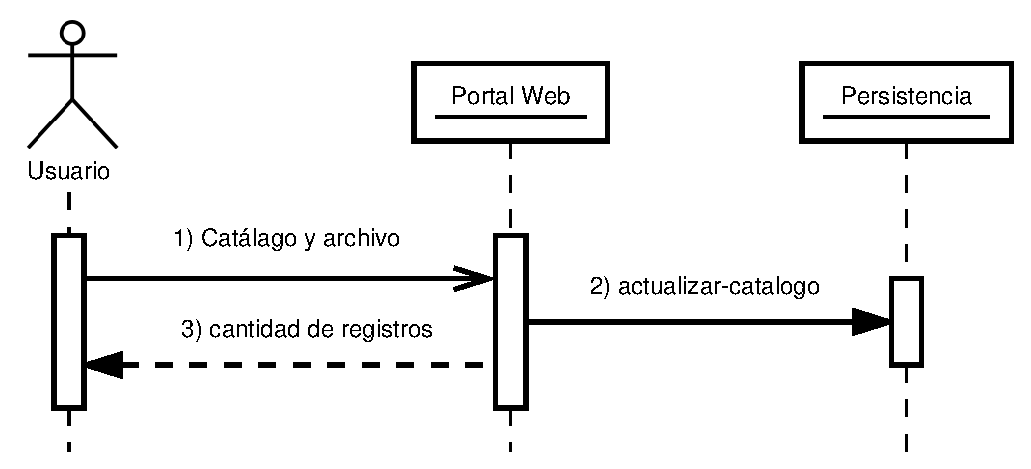
\includegraphics[scale=0.7]{dia-seq-cu-actualizar-catalogo}
	\caption{Diagrama de secuencia del caso de uso CU-ACTUALIZAR-CATALOGO.}
	\label{fig:dia-seq-cu-actualizar-catalogo}
\end{figure}

\subsubsection{Buscar órdenes}
El diseño de la solución al caso de uso \textbf{CU-BUSCAR} (sección \ref{cu-buscar}) se lleva a cabo entre el actor \textbf{Usuario} y los componentes \textbf{Portal Web} y \textbf{Persistencia} tal solución se logra realizando las siguientes llamadas (En el diagrama de la Figura \ref{fig:dia-seq-cu-buscar} se muestra el diagrama de secuencia):
\begin{enumerate}
	\item \textbf{Usuario}: llenada el formulario de búsqueda \textbf{filtro} (mensaje 1 del diagrama).
	\item \textbf{Portal Web}: pide la realización de la búsqueda de órdenes al componente \textbf{Persistencia} (mensaje 2 del diagrama).
	\item \textbf{Portal Web}: muestra al \textbf{Usuario} el listado de órdenes de reposición encontradas (mensaje 3 del diagrama).
\end{enumerate}

\begin{figure}[h]
	\centering
	\includegraphics[scale=0.7]{dia-seq-cu-buscar}
	\caption{Diagrama de secuencia del caso de uso CU-BUSCAR.}
	\label{fig:dia-seq-cu-buscar}
\end{figure}

\subsubsection{Visualizar orden}
El diseño de la solución al caso de uso \textbf{CU-VISUALIZAR} (sección \ref{cu-visualizar}) se lleva a cabo entre el actor \textbf{Usuario} y los componentes \textbf{Portal Web} y \textbf{Persistencia} tal solución se logra realizando las siguientes llamadas (En el diagrama de la Figura \ref{fig:dia-seq-cu-visualizar} se muestra el diagrama de secuencia):
\begin{enumerate}
	\item \textbf{Usuario}: selecciona la orden de reposición (mensaje 1 del diagrama).
	\item \textbf{Portal Web}: pide la realización de la búsqueda de la orden al componente \textbf{Persistencia} (mensaje 2 del diagrama).
	\item \textbf{Portal Web}: muestra al \textbf{Usuario} la información de la orden de reposición.
\end{enumerate}

\begin{figure}[h]
	\centering
	\includegraphics[scale=0.7]{dia-seq-cu-visualizar}
	\caption{Diagrama de secuencia del caso de uso CU-VISUALIZAR.}
	\label{fig:dia-seq-cu-visualizar}
\end{figure}

\subsubsection{Editar orden}
Ver sección \ref{cu-contestar}.\\
El diseño de la solución al caso de uso \textbf{CU-EDITAR} (sección \ref{cu-editar}) se lleva a cabo entre el actor \textbf{Usuario} y los componentes \textbf{Portal Web} y \textbf{Persistencia} tal solución se logra realizando las siguientes llamadas (En el diagrama de la Figura \ref{fig:dia-seq-cu-editar} se muestra el diagrama de secuencia):
\begin{enumerate}
	\item \textbf{Usuario}: activa la edición de la orden de reposición (mensaje 1 del diagrama).
	\item \textbf{Usuario}: modifica la información de la orden de reposición (mensaje 2).
	\item \textbf{Portal Web}: pide la actualización de la orden al componente \textbf{Persistencia} (mensaje 3 del diagrama).
\end{enumerate}

\begin{figure}[h]
	\centering
	\includegraphics[scale=0.7]{dia-seq-cu-editar}
	\caption{Diagrama de secuencia del caso de uso CU-EDITAR.}
	\label{fig:dia-seq-cu-editar}
\end{figure}


%===============================================================================
%===============================================================================

\newpage
\section{Diseño de la base de datos}
La base de datos tiene dos finalidades, guardar la información capturada de las órdenes de reposición atendidas así como los catálogos necesarios para los procesos automatizados y generación de reportes; la segunda es almacenar la información de los usuarios autorizados para utilizar el portal web.\\
El diseño de la base de datos se centra en los siguientes grupos\footnote{Los nombres de las tablas están escritos utilizando letras minúsculas de alfabeto inglés y guión bajo $([a-z]{\textunderscore})^+$}(ver Figura \ref{fig:dia-er-resumen}):
\begin{enumerate}
	\item Tablas de las órdenes de reposición.
	\item Tablas del registro de eventos.
	\item Tablas de los usuarios de la interfaz web.
	\item Catálogos para generación de reportes.
\end{enumerate}
\begin{figure}[h]
  \centering
  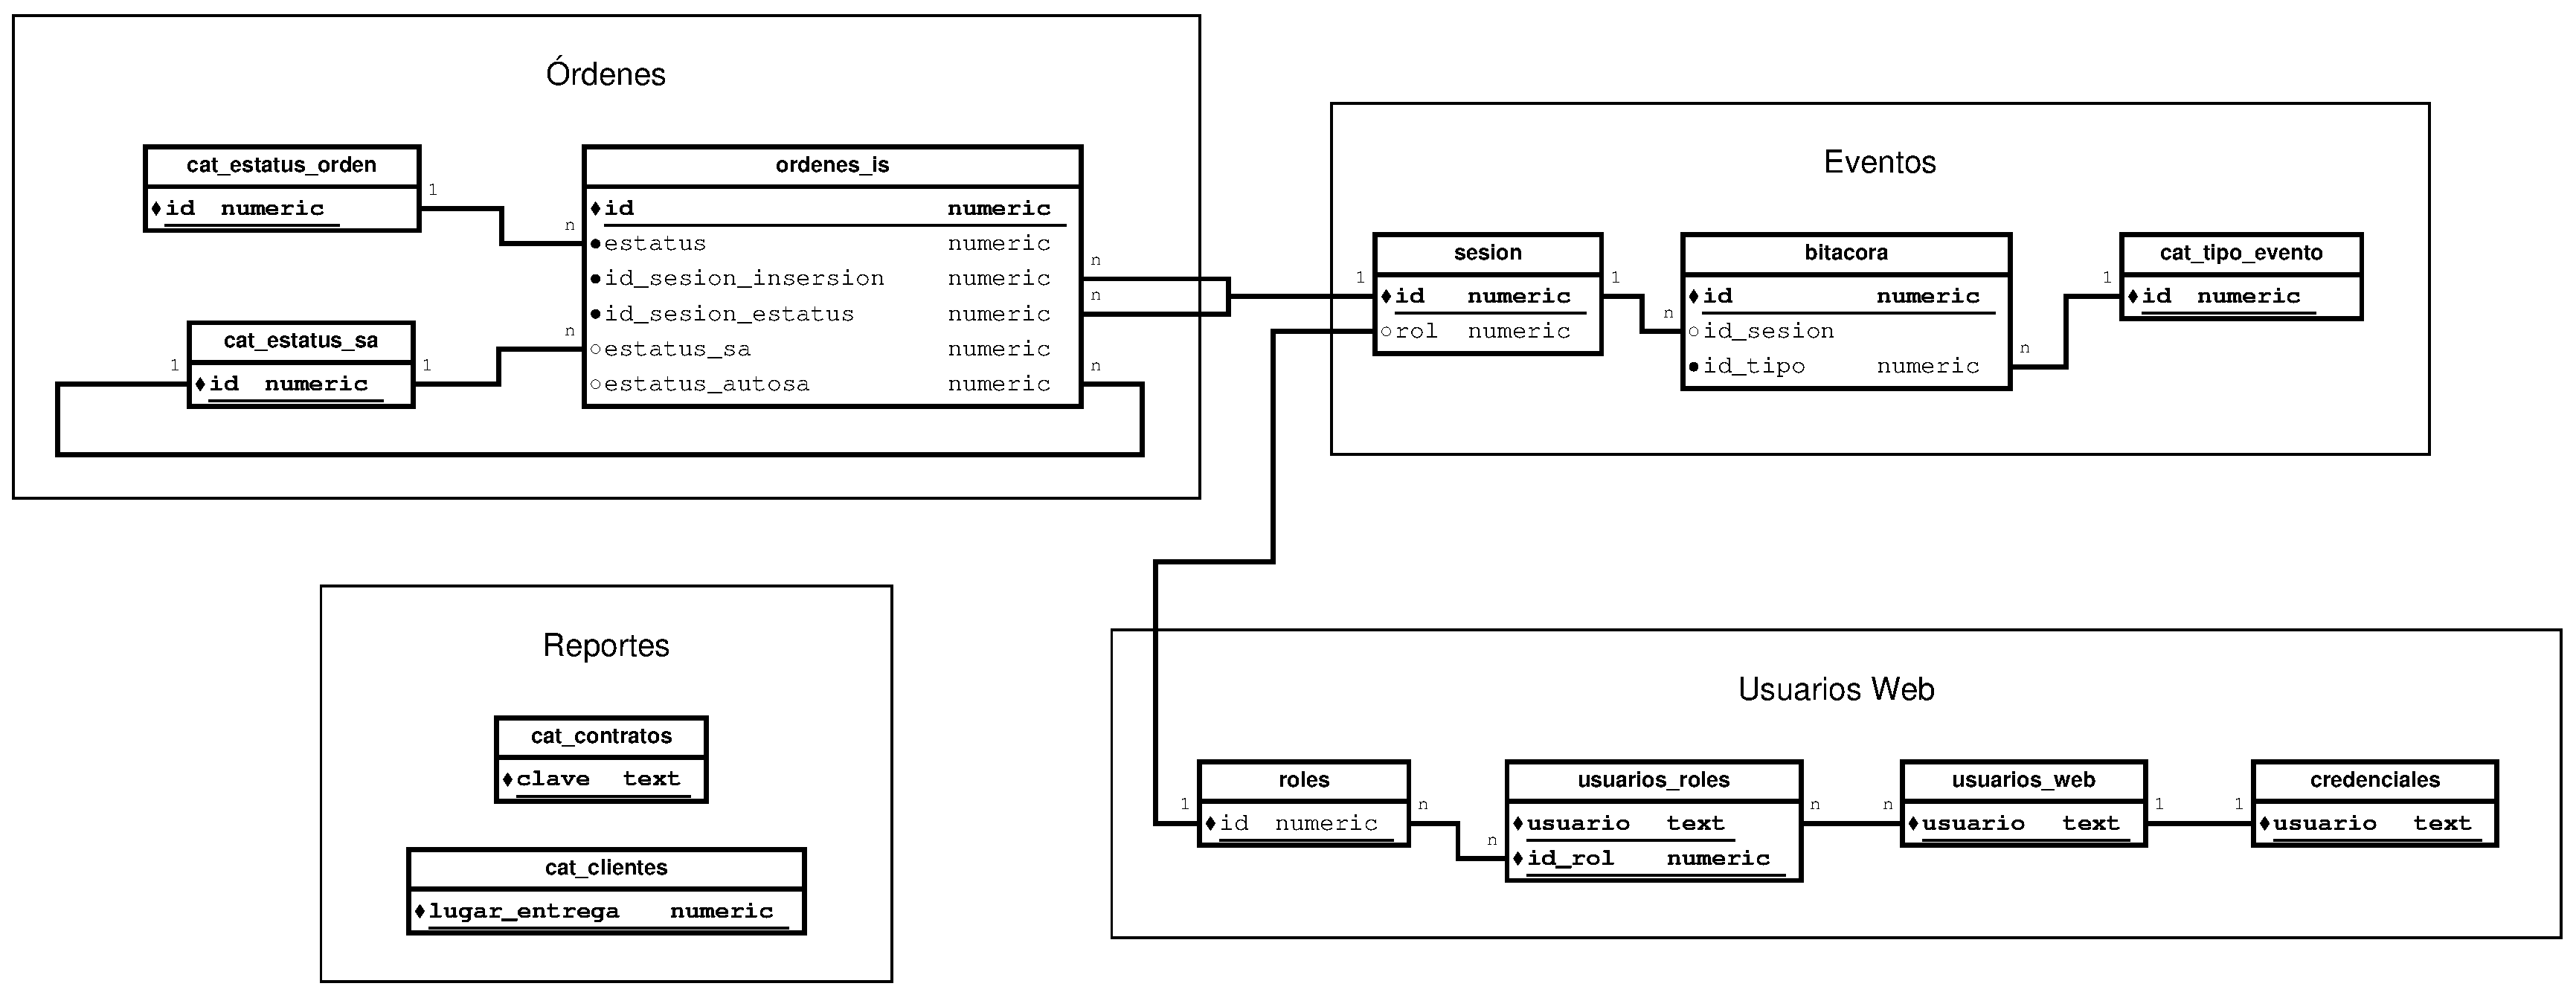
\includegraphics[width=\textwidth]{dia-er-resumen}
  \caption{Diagrama Entidad Relación de el Sistema AutoSA.}
  \label{fig:dia-er-resumen}
\end{figure}


\subsection{Tablas de las órdenes de reposición}
En estas tablas (ver Figura \ref{fig:dia-er-ordenes}) se almacenan las órdenes de reposición atendidas durante la rutina automatizada para responder órdenes de reposición en el Sistema de Abastecimiento\footnote{Ver caso de uso \ref{cu-contestar}}, de igual manera también es utilizada en la verificación de órdenes de reposición canceladas\footnote{Ver caso de uso \ref{cu-verificar}}.
\begin{figure}[h]
  \centering
  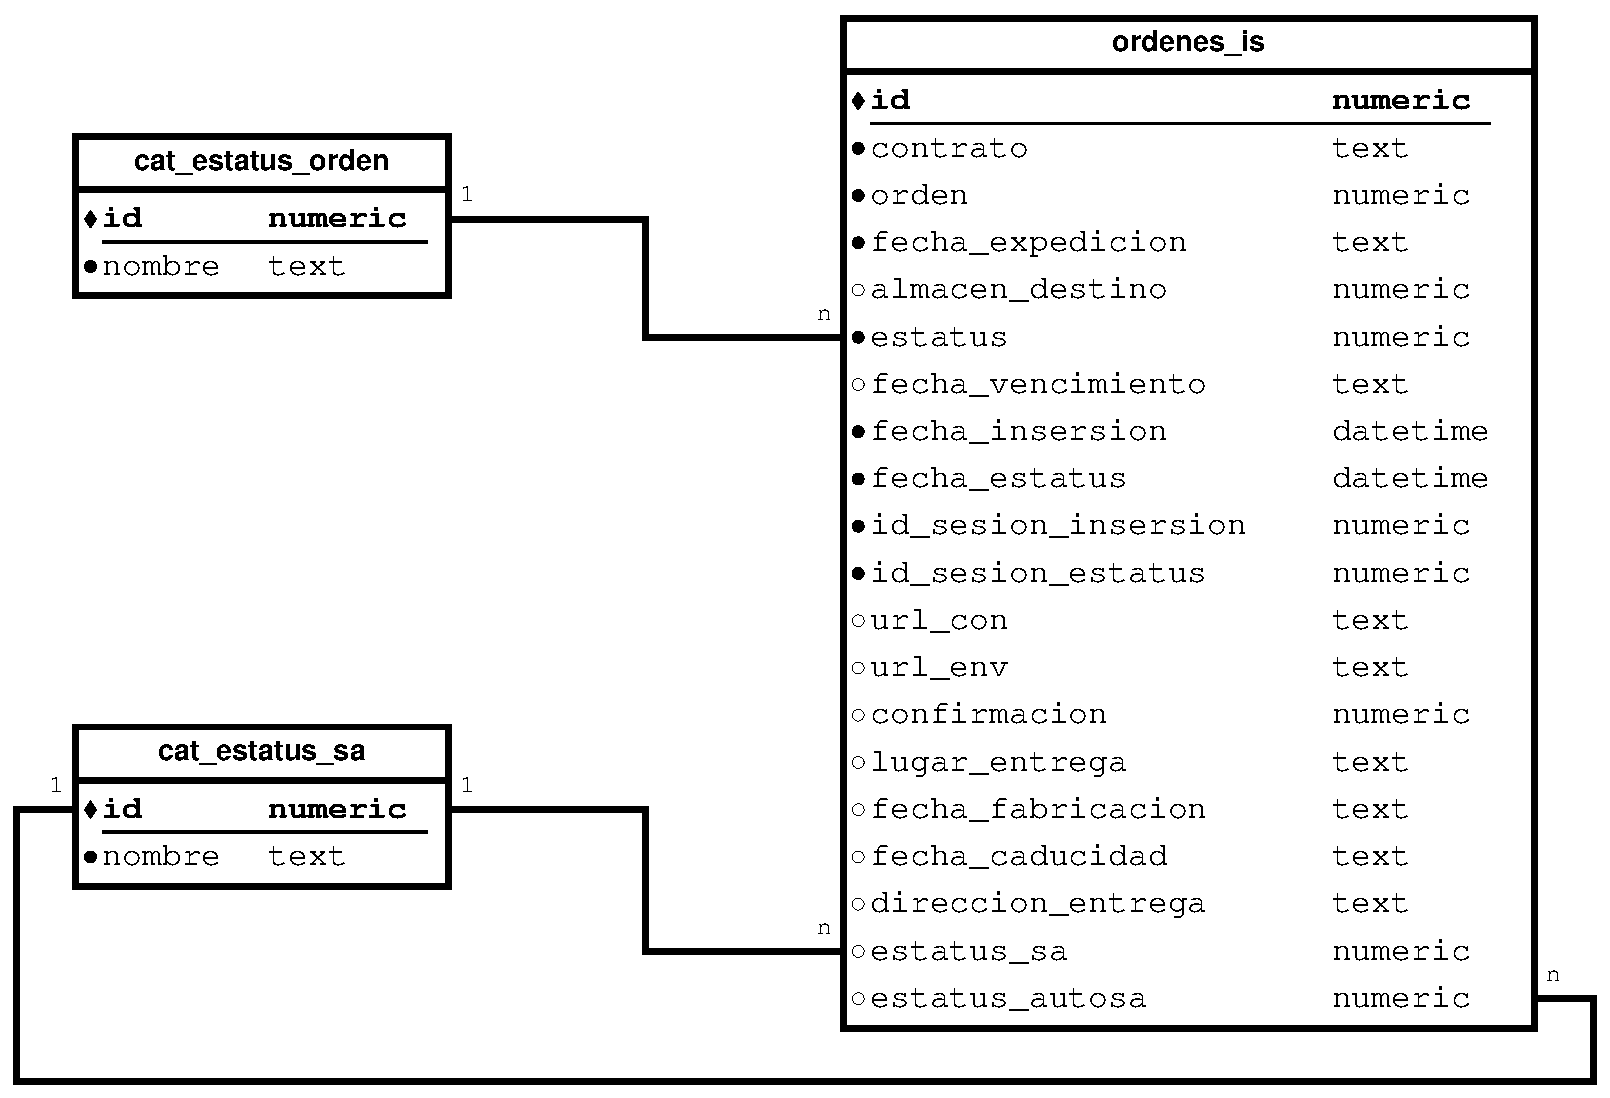
\includegraphics[scale=0.5]{dia-er-ordenes} 
  \caption{Diagrama Entidad Relación para el registro de órdenes de reposición.}
  \label{fig:dia-er-ordenes}
\end{figure}
\paragraph{ordenes{\textunderscore}is:} Contiene el registro de las órdenes de reposición del Sistema de Abastecimiento que han sido atendidas por la rutina de automatización.
\paragraph{cat{\textunderscore}estatus{\textunderscore}orden:} Este catálogo no debe ser alterado, contiene los posibles estatus que pude tomar una orden durante el ciclo de vida de la aplicación.
\paragraph{cat{\textunderscore}estatus{\textunderscore}sa:} Este catálogo contiene los estados definidos por el Sistema de Abastecimiento para registrar y almacenar una orden de reposición.


\subsection{Tablas del registro de eventos}
El registro de eventos es todo lo relacionado con actividad de los actores del sistema (agentes de automatización y usuarios), como se muestra en la Figura \ref{fig:dia-er-bitacora}.
\begin{figure}[h]
  \centering
  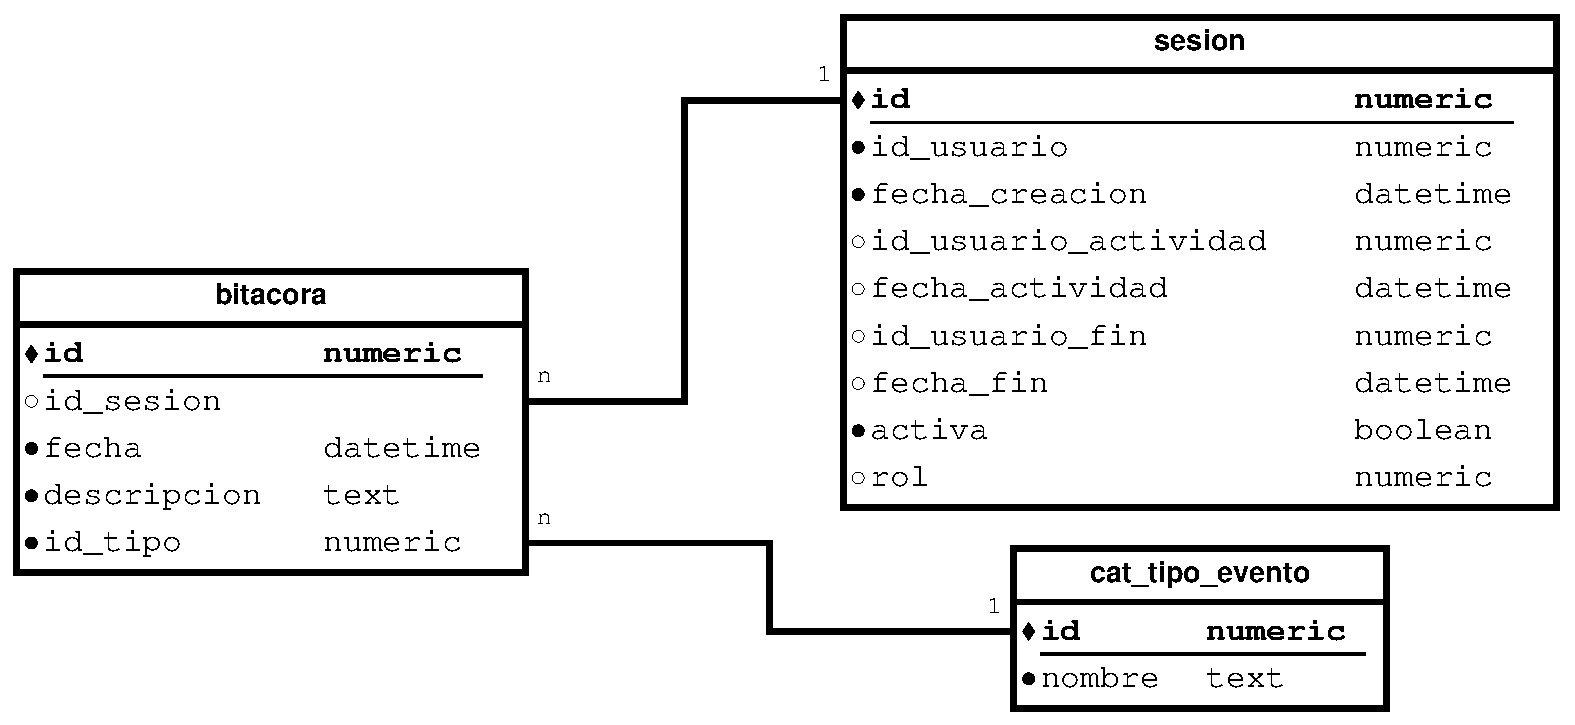
\includegraphics[scale=0.5]{dia-er-bitacora} 
  \caption{Diagrama Entidad Relación para el registro de eventos.}
  \label{fig:dia-er-bitacora}
\end{figure}
\paragraph{bitacora:} Lleva el registro de eventos ocurridos durante la ejecución de las rutinas de automatización, el evento puede estar ligado a una sesión.
\paragraph{cat{\textunderscore}tipo{\textunderscore}evento:} Catálogo con los tipos de eventos que pueden ser registrados en la bitácora.
\paragraph{sesion:} Define una sesión bajo la cual se ejecuta una rutina de automatización, la sesión puede definir implícitamente un usuario y un rol.


\subsection{Tablas de los usuarios de la interfaz web}
Las tablas de este grupo son utilizadas para gestionar el acceso a la interfaz web\footnote{Ver caso de uso \ref{cu-entrar-web}} (ver Figura \ref{fig:dia-er-web}).
\begin{figure}[h]
  \centering
  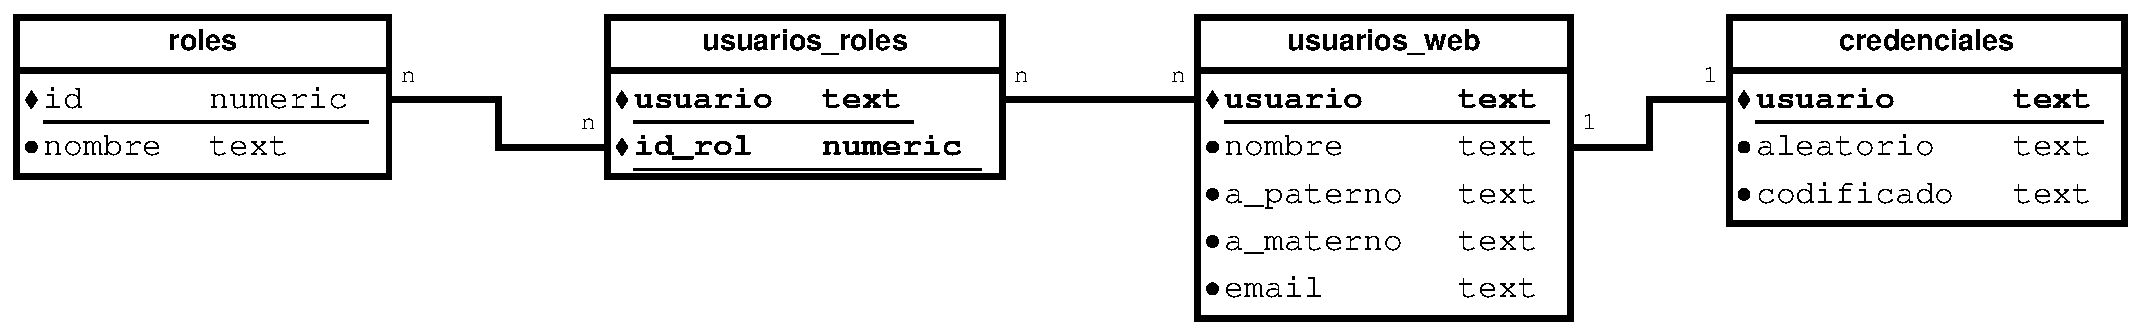
\includegraphics[scale=0.5]{dia-er-web} 
  \caption{Diagrama Entidad Relación para el manejo de usuarios.}
  \label{fig:dia-er-web}
\end{figure}
\paragraph{roles:}Contiene los roles (permisos) que los usuarios pueden tener en la interfaz web.
\paragraph{sesion:}Contiene información de las sesiones de los usuarios de la interfaz web.
\paragraph{usuarios{\textunderscore}web:} Contiene la información de los usuarios de la interfaz web.
\paragraph{credenciales:} Contiene la credenciales con las cuales los usuarios autentican su acceso a la interfaz web.


\subsection{Catálogos para la generación de reportes}
Estas tablas contienen catálogos (ver Figura \ref{fig:dia-er-reportes}) que son necesarios para la generación de los reportes\footnote{Ver casos de uso \ref{cu-generar-reporte} y \ref{cu-actualizar-catalogo}} que sirven que las siguientes áreas de la farmacéutica continúen con la atención de las órdenes de reposición.
\begin{figure}[h]
  \centering
  \includegraphics[scale=0.5]{dia-er-reportes} 
  \caption{Diagrama Entidad Relación de los catálogos para la generación de vistas.}
  \label{fig:dia-er-reportes}
\end{figure}
\paragraph{cat{\textunderscore}clientes:} Este catálogo contiene información sobre la localización física de los lugares donde deben ser entregados los productos.
\paragraph{cat{\textunderscore}contratos:} Este catálogo contiene información referente a acuerdos comerciales referentes a los productos requeridos en las órdenes de reposición.


\section{Resumen}
En este capítulo se ha mostrado la arquitectura del Sistema AutoSA, los componentes del mismo y las interfaces que ofrecen. Posteriormente se ha mostrado el flujo de mensajes entre los componentes del sistema para llevar a cabo los casos de uso del Capítulo \ref{cap2}. Así mismo se ha modelado la base de datos que a grandes rasgos está destinada a almacenar información de las órdenes de reposición e información de los usuarios del Sistema AutoSA.\\
El diseño planteado será implementado en el siguiente capítulo donde se verá a detalle el funcionamiento de cada módulo así como algoritmos, tecnologías y marcos de trabajo utilizados. 